\section{Exempelskript för ickelinjär kurvanpassning}
\label{sec:matlab-nonlinear}
I detta exempel finner ni ett Matlab skript ({\tt passning.m}) för
ickelinjär kurvanpassning. Ekvationen som passas i exemplet är helt godtycklig:

\begin{equation}
  \label{eq:ex}
  f(x) = a\frac{x^b+1}{x^{b+1}+1}
\end{equation}

\begin{figure}
  \centering
  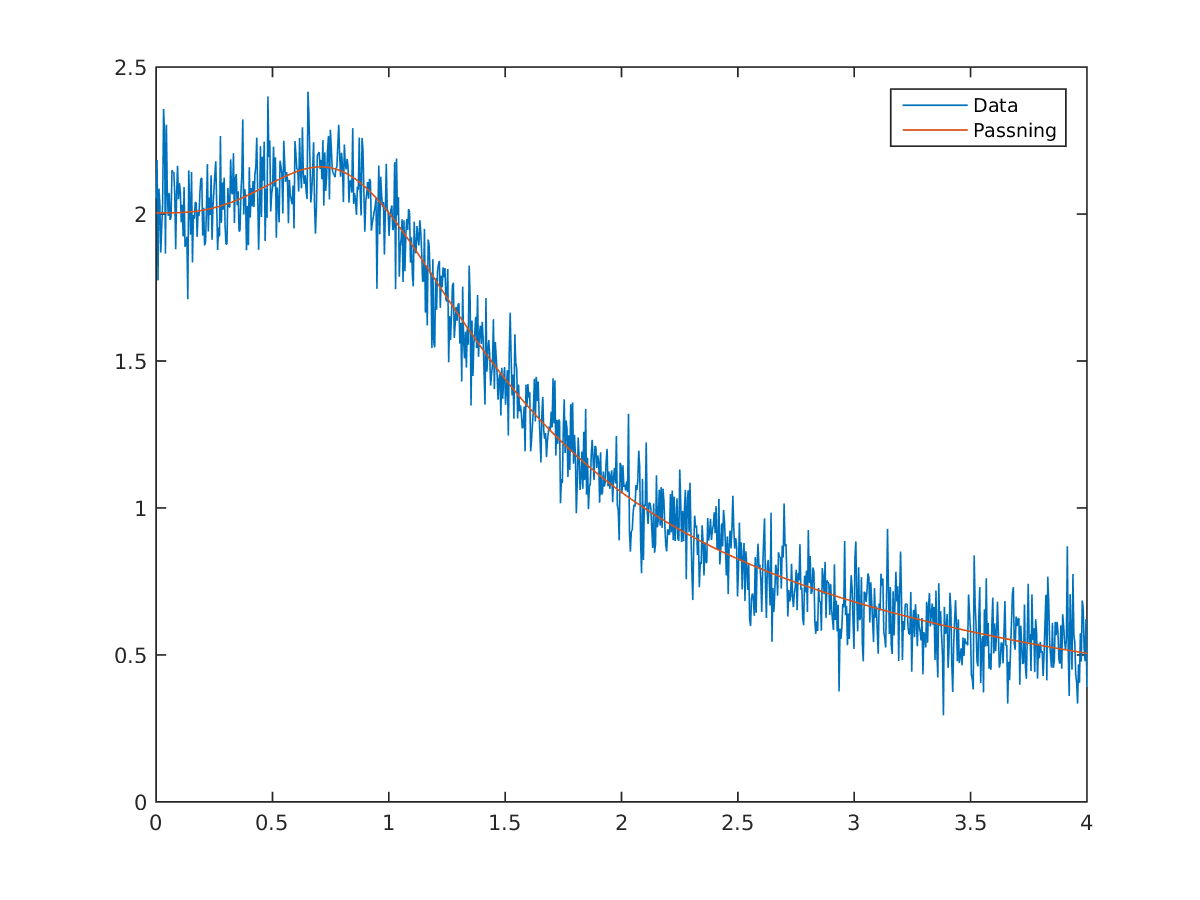
\includegraphics[scale=0.5]{matlab/passning.png}
  \caption{Ickelinjär kurvanpassning}
  \label{fig:matlab-nonlinear}
\end{figure}

Vi genererar data med en relativt hög brusnivå (se
\cref{fig:matlab-nonlinear}) för att utmana passningsrutinen. Därefter
optimerar vi (utifrån en startgissning) värden på $a$ respektive $b$,
först med Matlabs funktion {\tt fsolve} (se \cref{sec:matlab-fsolve}) och
sedan en alternativ version med Matlabs funktion {\tt fit} (se
\cref{sec:matlab-fit}).

\subsection{Kod baserad på ``fsolve''}
\label{sec:matlab-fsolve}
{\tt fsolve} kan ansättas att försöka lösa en ekvation för
residualerna för vår passning ($\vec{r}(\vec{x}) = \vec{0}$).

\begin{equation}
  \label{eq:ex}
  r_i(x_i) = a\frac{x_i^b+1}{x_i^{b+1}+1} - y_i
\end{equation}

\matlabcode{matlab/passning2.m}

\begin{terminaloutput}
>> passning2
Warning: Trust-region-dogleg algorithm of FSOLVE cannot handle non-square systems; using Levenberg-Marquardt algorithm instead. 
> In fsolve (line 287)
  In passning2 (line 43) 

No solution found.

fsolve stopped because the last step was ineffective. However, the vector of function
values is not near zero, as measured by the default value of the function tolerance. 

<stopping criteria details>


result =

    2.0015    2.9760
\end{terminaloutput}
{\tt fsolve} föreslår alltså värden för $a$ och $b$ nära våra valda
korrekta värden ($\alpha$ och $\beta$).

\subsection{Kod baserad på {\tt fit}}
\label{sec:matlab-fit}
Metoden med {\tt fsolve} ger inga konfidensintervall, 
samt varnar för det mesta (om inställningar inte
görs aktivt) att efterfrågade toleranser inte kunde uppnås.
{\tt fit} ger likvärdiga passningar men ger både konfidensintervall och
har mer ändamålsenliga varningar. Använd den metod ni är mest bekväma med
-- antingen {\tt fsolve} eller {\tt fit}.

\matlabcode{matlab/passning.m}

När vi exekverar koden ovan får vi följande utdata i terminalen:

\begin{terminaloutput}
>> passning

fitobj = 

     General model:
     fitobj(x) = (a*g(b,x)./g(b+1,x))
     Coefficients (with 95% confidence bounds):
       a =       2.004  (1.988, 2.02)
       b =       3.207  (2.813, 3.601)

standard_deviation =

    0.0082    0.2009


root_mean_square_error =

    0.0999
\end{terminaloutput}

Vi ser att passningen lyckades och de sanna värdena ligger väl inom
angivna 95\%  konfidensintervall. Vi noterar dock att osäkerheten är
relativt stor för {\tt b}. Observera att vi gav startvärdena 1 för
optimeringen av $a$ och $b$. För att kurvanpassningen skall vara pålitlig
bör man försöka välja så bra startvärden som möjligt. Genom att titta på
den brusiga kurvan i \cref{fig:matlab-nonlinear} kunde vi t. ex. från
skärningspunkten med y-axeln satt startgissningen för $a$ någonstans
kring 2 och sedan löst ut $b$ ur en approximativ version av \cref{eq:ex} för
$f(4) \approx 0.5$.

%%% Local Variables:
%%% mode: latex
%%% TeX-master: "../main"
%%% ispell-local-dictionary: "swedish"
%%% End:
